\subsubsection{Microbenchmarks against Graph Databases}

We follow the AsterDB artifact methodology, running 100\,K single-threaded operations per measurement on DBLP (${\sim}317$\,K vertices, 1.05\,M edges) and Wikipedia (${\sim}1.87$\,M vertices, 4.51\,M edges).

\textbf{Structural operations.}
\autoref{fig:structural-ops} reports single-operation latencies for four core graph mutations.
On DBLP, \project{} Adjacency~List retrieves neighbors in 1.17\,$\mu$s, $10\times$ faster than Neo4j (11.67\,$\mu$s) and $27\times$ faster than AsterDB (31.42\,$\mu$s).
Vertex insertion takes 1.88\,$\mu$s vs.\ Neo4j's 8.75\,$\mu$s ($4.7\times$).
Edge insertion and deletion are competitive: \project{} EdgeKey deletes an edge in 6.59\,$\mu$s, $2\times$ faster than AsterDB (13.32\,$\mu$s) and $3.4\times$ faster than Neo4j (22.09\,$\mu$s).
Document-oriented systems (ArangoDB at 43\,ms for \code{get\_neighbors}, OrientDB at 20\,ms) are 3--4~orders of magnitude slower due to per-operation document serialization.
On the larger Wikipedia graph, \project{} retains its read advantage ($2.10$\,$\mu$s vs.\ Neo4j's $55.4$\,$\mu$s for \code{get\_neighbors}) and remains competitive on mutations.

%%%%%%%%%%%%%%%%%%%%%%%%%%%%%%%%%%%%%%%%%%%%%%%%%%%%%%%%%%%%%%%%%%%%%%%%%%%%%%%%
\begin{figure}[t]
  \centering
  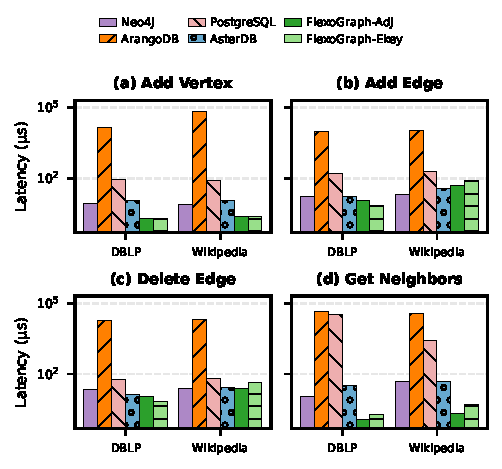
\includegraphics[width=\columnwidth]{content/fig/property/structural_ops.pdf}
  \caption{Single-operation structural latencies ($\mu$s, log scale) on DBLP and Wikipedia datasets. Lower is better.}
  \label{fig:structural-ops}
\end{figure}
%%%%%%%%%%%%%%%%%%%%%%%%%%%%%%%%%%%%%%%%%%%%%%%%%%%%%%%%%%%%%%%%%%%%%%%%%%%%%%%%

\textbf{Property mutations.}
\autoref{fig:property-crud} reports eight property CRUD operations on the artifact's LDBC and Freebase datasets.
For fine-grained mutations (update, insert, delete), \project{} and AsterDB are 3--4~orders of magnitude faster than systems with a query-language layer.
On the LDBC dataset, \project{} updates a vertex property in $0.01$\,ms (${\sim}10$\,$\mu$s); AsterDB takes $0.05$\,ms; Neo4j takes 46.7\,ms; JanusGraph 105.8\,ms.
Neo4j's cost is almost entirely overhead: parsing a Groovy script, resolving the element by label-property index, and writing through its transactional record store, while \project{} issues a single \wt{} cursor \code{update} call.
For property search (scanning all vertices or edges for a value match), \project{} Adjacency~List completes vertex search in 14.4\,ms, $21\times$ faster than AsterDB (303\,ms) and $29\times$ faster than Neo4j (425\,ms).

%%%%%%%%%%%%%%%%%%%%%%%%%%%%%%%%%%%%%%%%%%%%%%%%%%%%%%%%%%%%%%%%%%%%%%%%%%%%%%%%
\begin{figure*}[t]
  \centering
  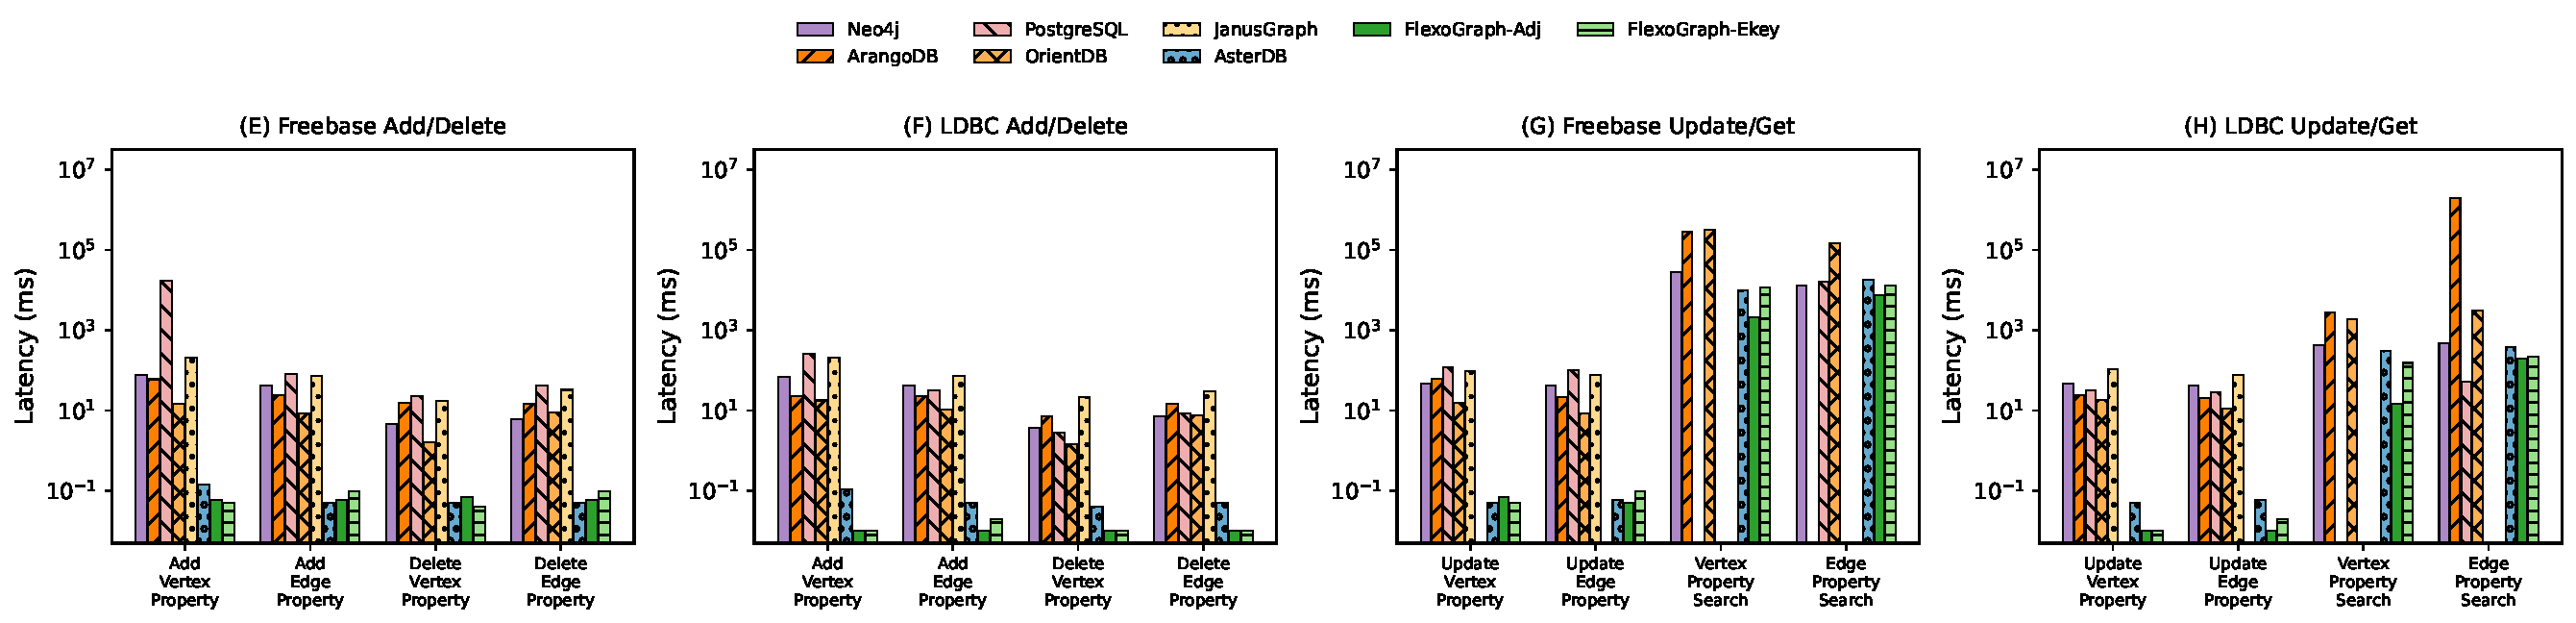
\includegraphics[width=\textwidth]{content/fig/property/property_crud.pdf}
  \caption{Property CRUD operation latencies (ms, log scale) on the Freebase and LDBC datasets. Eight operations: add/delete/update vertex and edge properties, plus vertex and edge property search. Lower is better.}
  \label{fig:property-crud}
\end{figure*}
%%%%%%%%%%%%%%%%%%%%%%%%%%%%%%%%%%%%%%%%%%%%%%%%%%%%%%%%%%%%%%%%%%%%%%%%%%%%%%%%
% NEED TO MENTION THIS: We exclude AsterDB from the LDBC comparison: although its RocksDB backend persists properties, the Gremlin bridge reads vertex properties from an in-memory map that is never populated from storage, so property lookups return null; additionally, all edges are stored under a single default label, preventing label-filtered traversals.
% AsterDB's property write path and indexed \code{has()} lookups are fully wired, so it participates in the CRUD microbenchmarks.